\subsection{Testing Framework}

After exploring a set of options to test this idea, the best place to go was to the drawing
board. Taking a step back it was decided that pushing to get straight into hardware testing
was a poor decision and the underlying concept of heterogeneous task reallocation based on
capabilities needed to be tested at the lowest of levels. To do this, the creation of a testing
framework in roscpp was necessary. The primary components of this system include the physical entities,
motion model, robot addition, robot.run() and the simulated verbose map,. The system has each robot
running individually, only communicating with neighbors through subscription and publication
to topics that are necessary to implement cooperation. This allows for testing of a completely
decentralized algorithm in a centralized system, giving algorithmic and cooperation designs
the primary focus while abstracting out complicated sensor models. This system started to take
shape this over the course of the past few months when trying to use third party multimaster
implementations in Gazebo, which turned out to necessitate the experiment be running on multiple
computers.

The major components of the testing framework that I designed include an Entity class with Neighbor and Robot derived class, a map class
that holds the obstacle information and can be queried based on a sensing radius, and the main loop.
The use of C++ templates and proper organization according to ROS best practices, this testing framework
can be utilized for far more than this project alone, and was all written from scratch \cite{ROS}.

\subsubsection{Entities}

The Entity class is the base physical structure for this testing package. This could represent a static
or one of the two derived classes: Neighbor and Robot. Entities hold major variables like state
information, initial position and odometry. The Neighbor and Robot classes are very similar to each other
as they both represent robots, the Neighbor class is just used to hold the information for the
Robot's neighboring robots as they do not need to keep track of their entire path and known map,
like they are doing for themselves.

\subsubsection{Motion Model}

The motion model is pretty simple, but is by far the hardest to get right for all robot systems. This
portion would often necessitate the user to implement some helper methods to properly used the simple
motion primitives that each Robot has as a few class functions like goLeft(), goRight, go(float3), etc.
Regardless, the main way to ensure that control is occurring properly. One feature that would allow
for easier handling of this would be the yaml config files that are briefly discussed in the next section.

\subsubsection{Adding Robots}

This framework allows for easy addition of robots by simply
adding the details for the new robot in the xml robots launch file. To add any additional information
yaml files can be used to set rosparams and can be queried in any rosnode as long as the yaml file
was specified in one of the launch files as a rosparam. Utilization of the yaml files is essential
to adding and sharing information like hardware characteristics before Robots enter the main loop. So all in all, By configuring
the launch file with the proper robots, one can edit the one robot launch file to have each robot launch
any set of nodes that would exist in each robot's namespace.

One thing that was essential to streamline and allow for flexibility was the instantiation of robots via partitioned
launch files. By defining separate roslaunch files instead of one, it is easy to see where to
put new robots as well as ensure that one point of failure is taken care of.
The one robots launch file launches nodes that are to be in every robot,
who are defined by namespaces in the context of ROS. The robots launch file is where robot descriptions
are set along with locations of urdf files containing meshes and other simulation specific
data for the individual robot. The launch file can be called by a users custom
launch file; in our case this was the hare sim launch file.

As can be seen in the figure at the top of this document tests were conducted with a Husky bot, rosbot, and youbot. The Husky bot is more of a heavy duty autonomous vehicle with a wide range of terrain capabilities. The rosbot is a
small robot that is generally used for testing and eduction. Finally, the youbot which may be the most
interesting of the bunch as it has holonomic capabilities due to having the well know swiss wheels.

\subsubsection{Robot.run()}

Due to this being a decentralized testing system, even though it is actually
centralized, all robots must be able to operate autonomously. This is accomplished
by all robots running the same main loop and keeping their neighbors aware of where they were
in the operational lifetime as well as if help is needed from a fellow agent. This loop can be seen
below in ~\ref{fig:HARE} after the first direction assignment has been determined and is
located solely in the method robot.run().


\begin{figure}[H]
  \centering
    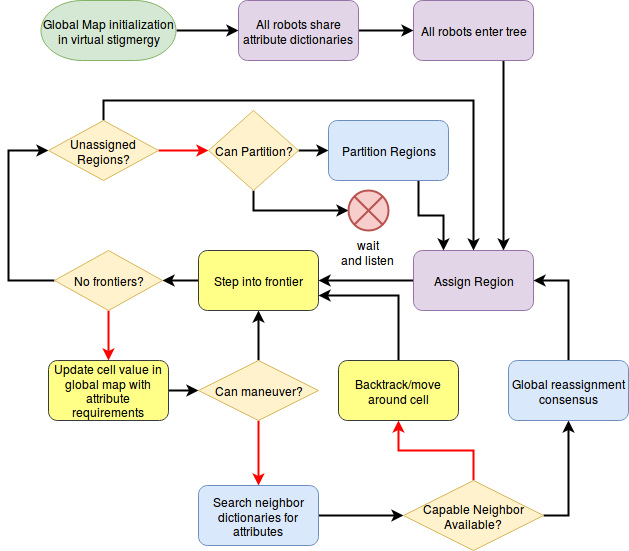
\includegraphics[width=0.75\textwidth]{HARE}
  \caption{High level block diagram for HARE}
  \label{fig:HARE}
\end{figure}

\subsubsection{Simulated Map}

The simulated map is essential to testing as it allows for user defined obstacles as well as the
potential to expand into randomly generated maps. This map is a static NxN array of map nodes which
hold information like cell terrain, if the cell had been explored, edge characteristics, and more.
The usefulness of a map like this comes from the ability to self define edge cases as well as not
have to worry about a complicated mapping and sensing scheme. This could obviously not be used
in the real world, but is great for testing. Even though the entire map exists in the software,
robots cannot simply access this map, they can only access a certain radius around them called their
sensed region. Each robot will update its known map whenever new cells are sensed and will also
transmit those cells to their neighbors to maximize exploration and global coverage. The first map
that this system utilizes can be seen below in 2D in ~\ref{fig:2D} as well as 3D in ~\ref{fig:3D1}
and ~\ref{fig:3D2}.

\begin{figure}[H]
    \begin{center}
    \begin{subfigure}[b]{0.45\textwidth}
        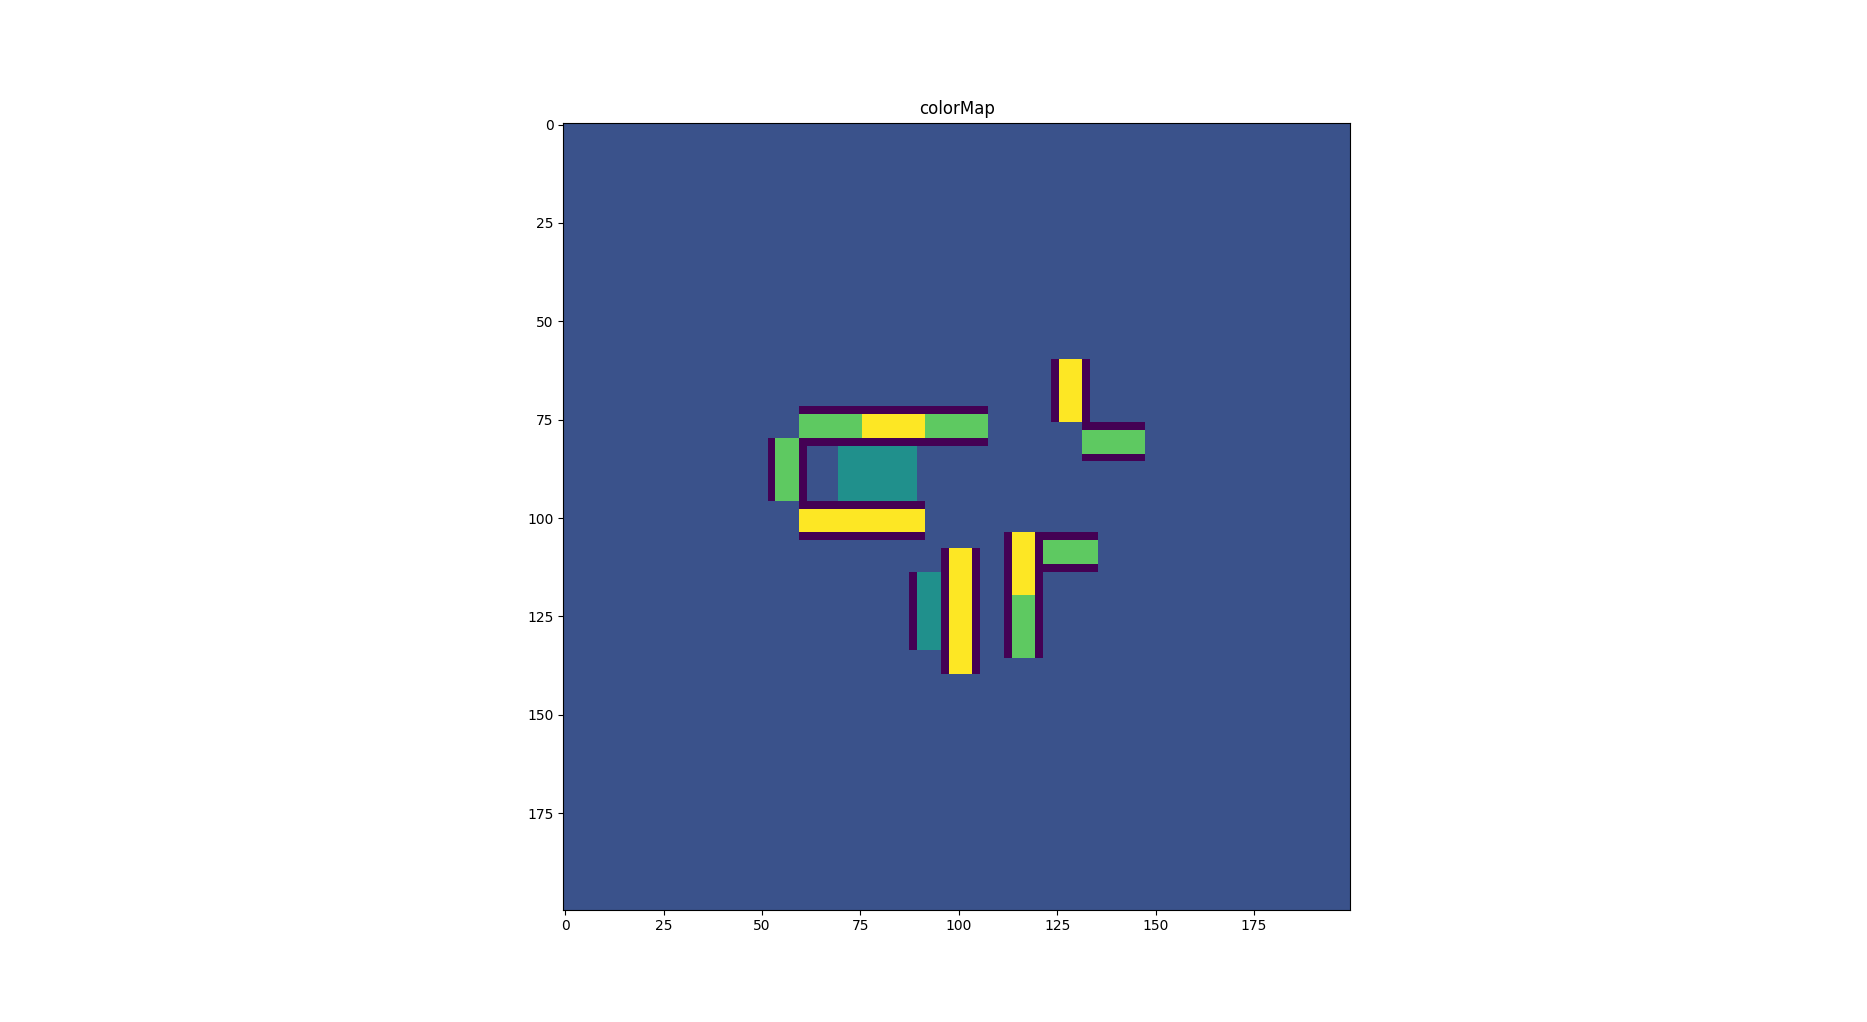
\includegraphics[width=\textwidth]{2DHAREMap}
        \caption{2D view of HARE test map}
        \label{fig:2D}
    \end{subfigure}
    \begin{subfigure}[b]{0.25\textwidth}
        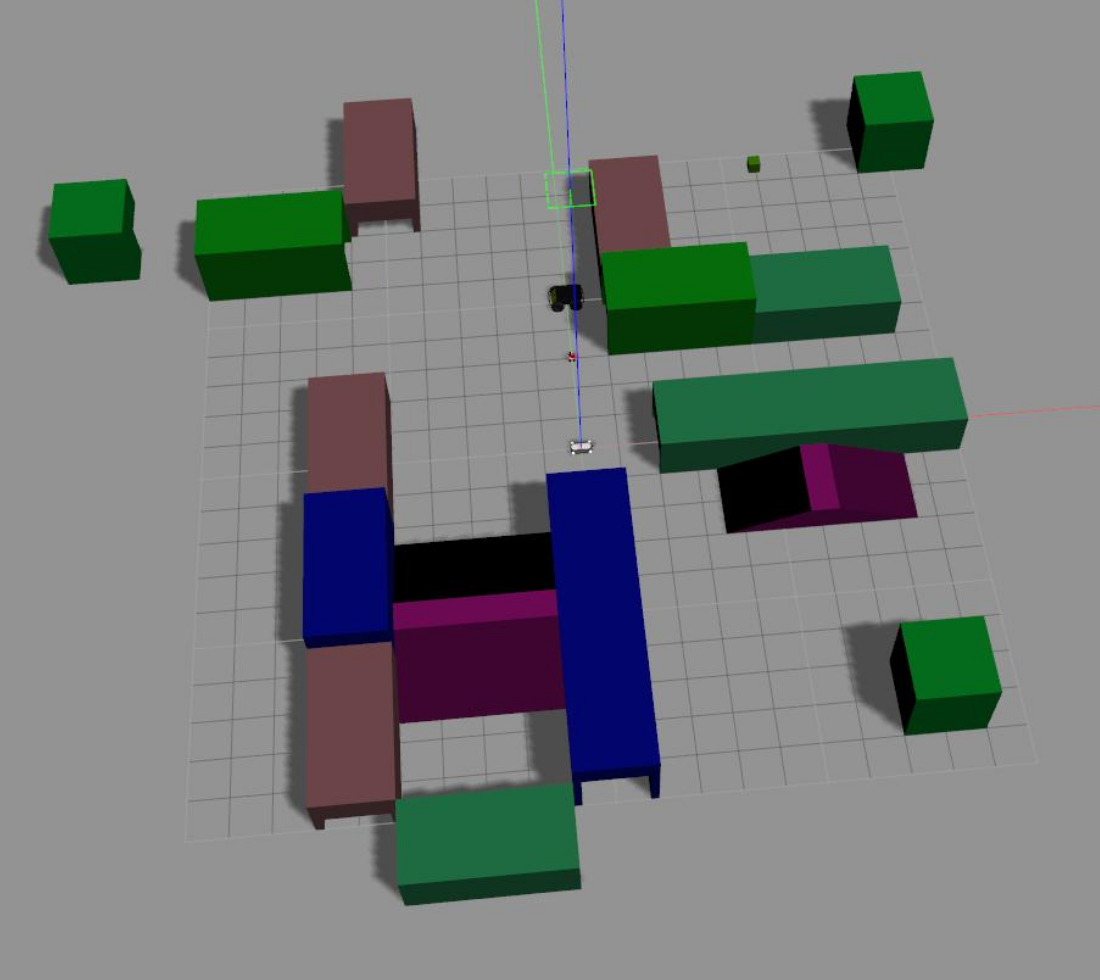
\includegraphics[width=\textwidth]{map2}
        \caption{Hare Map angle a}
        \label{fig:3D1}
    \end{subfigure}
    \begin{subfigure}[b]{0.25\textwidth}
        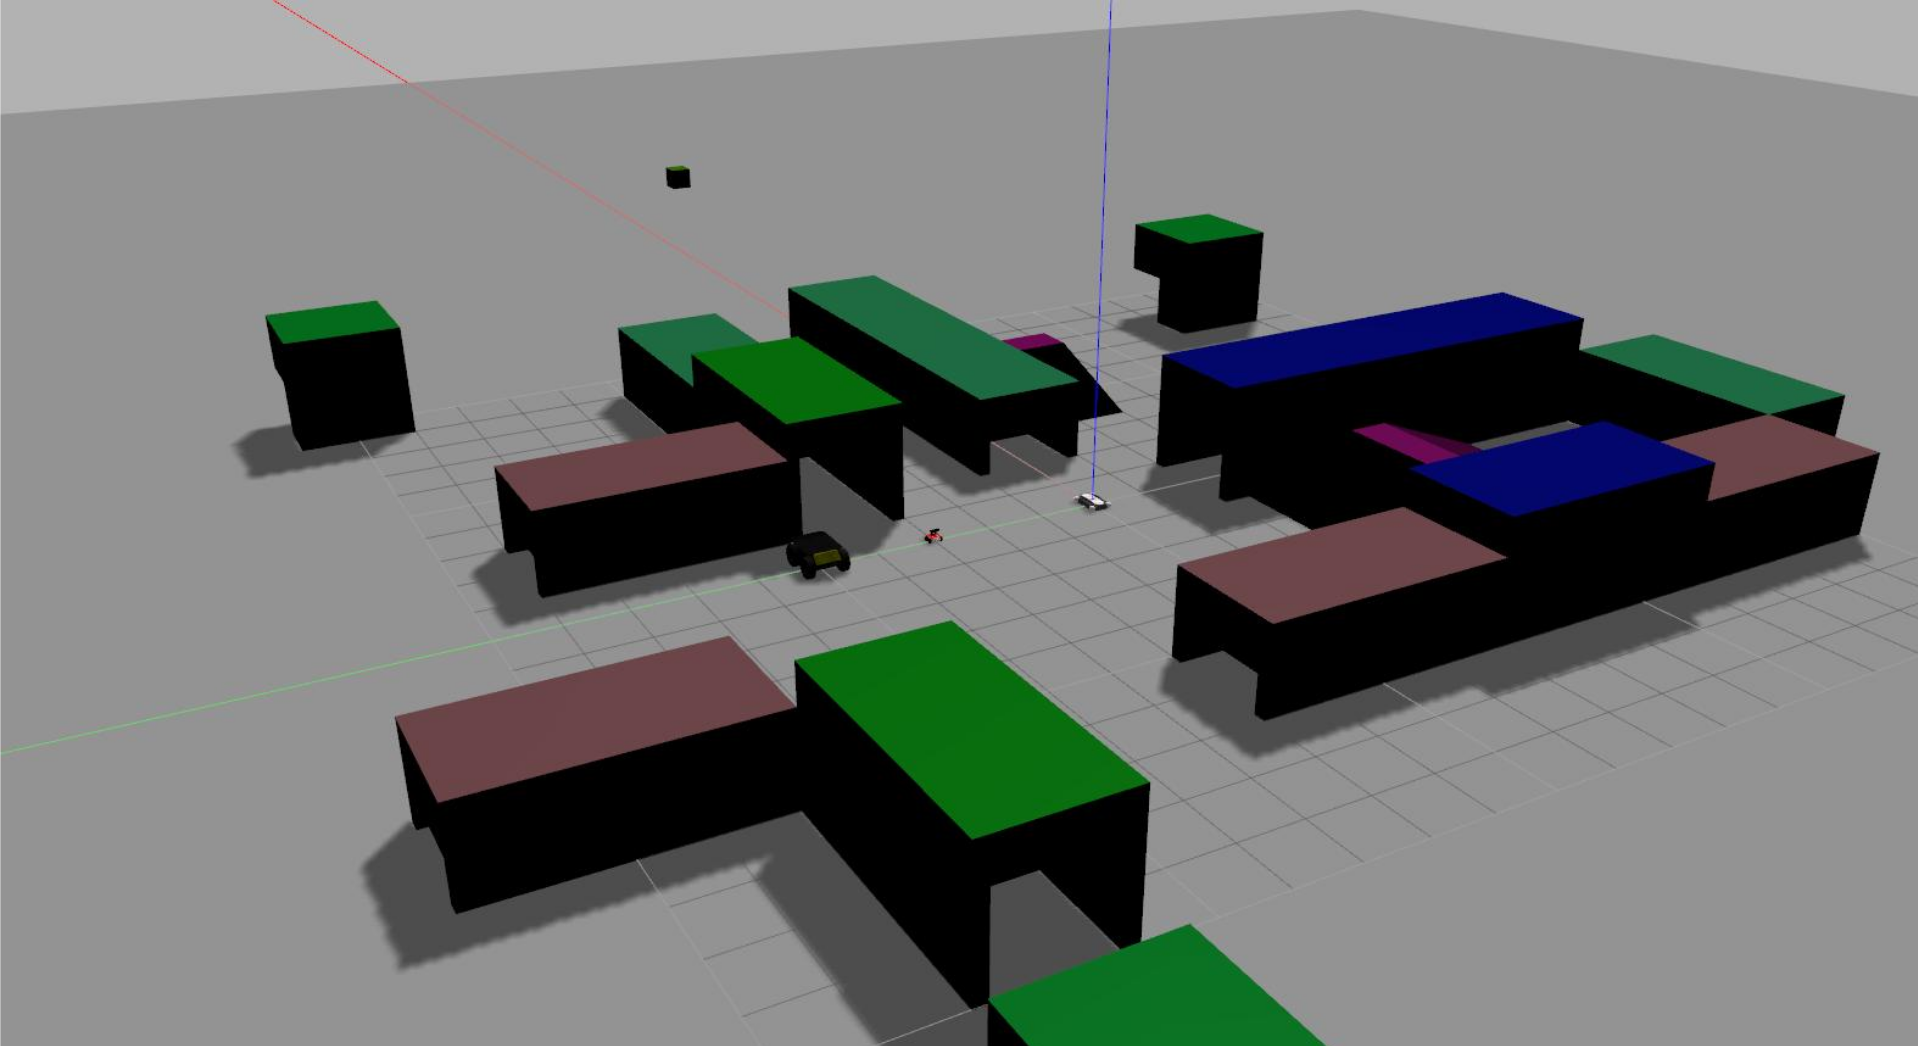
\includegraphics[width=\textwidth]{map1}
        \caption{Hare Map angle b}
        \label{fig:3D2}
    \end{subfigure}
  \end{center}
\end{figure}


\subsection{Algorithms}

Even though the algorithms in this system became less of a focus,
the usage of a custom weighted Depth First Search was designed as well as a
heuristic based path planning approach called Greedy Best First.

\subsubsection{DFS}

Psuedo code for the designed "DFS" algorithm can be seen below:

\begin{algorithm}[H]
\begin{algorithmic}[1]
\caption{Custom MRS Weighted DFS}
\State Let: $map = \{cell_\text{x,y,ownerID} \in R^{2}\}$
\State Let: $path = \{cells \in map_\text{visited} | length \leq maxPathLength\}$
\State Let: $weights = \{neighbor,groupCentroid,xy\}$
\newline
\Procedure{OVERALL STEP FUNCTION}{}
\BState \emph{\textbf{recvUpdates}}:
  \State $neighborInfo \gets robot_i.update$
  \State $map_\text{x,y} \gets robot_i.id$
\BState \emph{\textbf{checkForStopCriteria}}:
  \If {$length(group) == length(Robots) \text{ } \&\& \text{ } self.cell == leader.cell$} \Return
  \EndIf
\BState \emph{\textbf{refineGroup}}:
\BState \emph{\textbf{computeOptions}}:
\BState \emph{\textbf{move}}:
  \State $checkFreedom()$
  \State $checkForPause()$
  \State $sortDirections()$
  \For{$rankedDirections \in possibleDirections$}
    \If {$self.backTrack$} break
    \EndIf
    \If {$cell_\text{t+1}.ownerID != self.id$}
      \State $group.add(cell_\text{t+1}.ownerID)$
      \State $move()$
    \EndIf
  \EndFor
  \If {$hasNotMoved$}
    \State $backTrack()$
    \State $self.backTrack = false$
  \EndIf
\BState \emph{\textbf{checkForSuccessCriteria}}:
  \If {$length(group) == length(Robots) \&\& euclideanDistance(robot_i, self) == 0$}
    \State $success = true$
    \State $exit()$
  \EndIf

\EndProcedure
\end{algorithmic}
\end{algorithm}


\subsubsection{Greedy Best First Search}

In addition to DFS, Greedy Best First Search algorithm was implemented to derive a
possible path to a certain location in the map \cite{GBF}. In ~\ref{fig:gbf} one can see the
path from one point to another being highlighted. This algorithm is not the best
for path planning but was thought to be sufficient for the design with this test, not
to mention much of the focus had to be shifted the design of the testing package after
losing time to technology option rabbit-holes.

\begin{figure}[H]
  \centering
    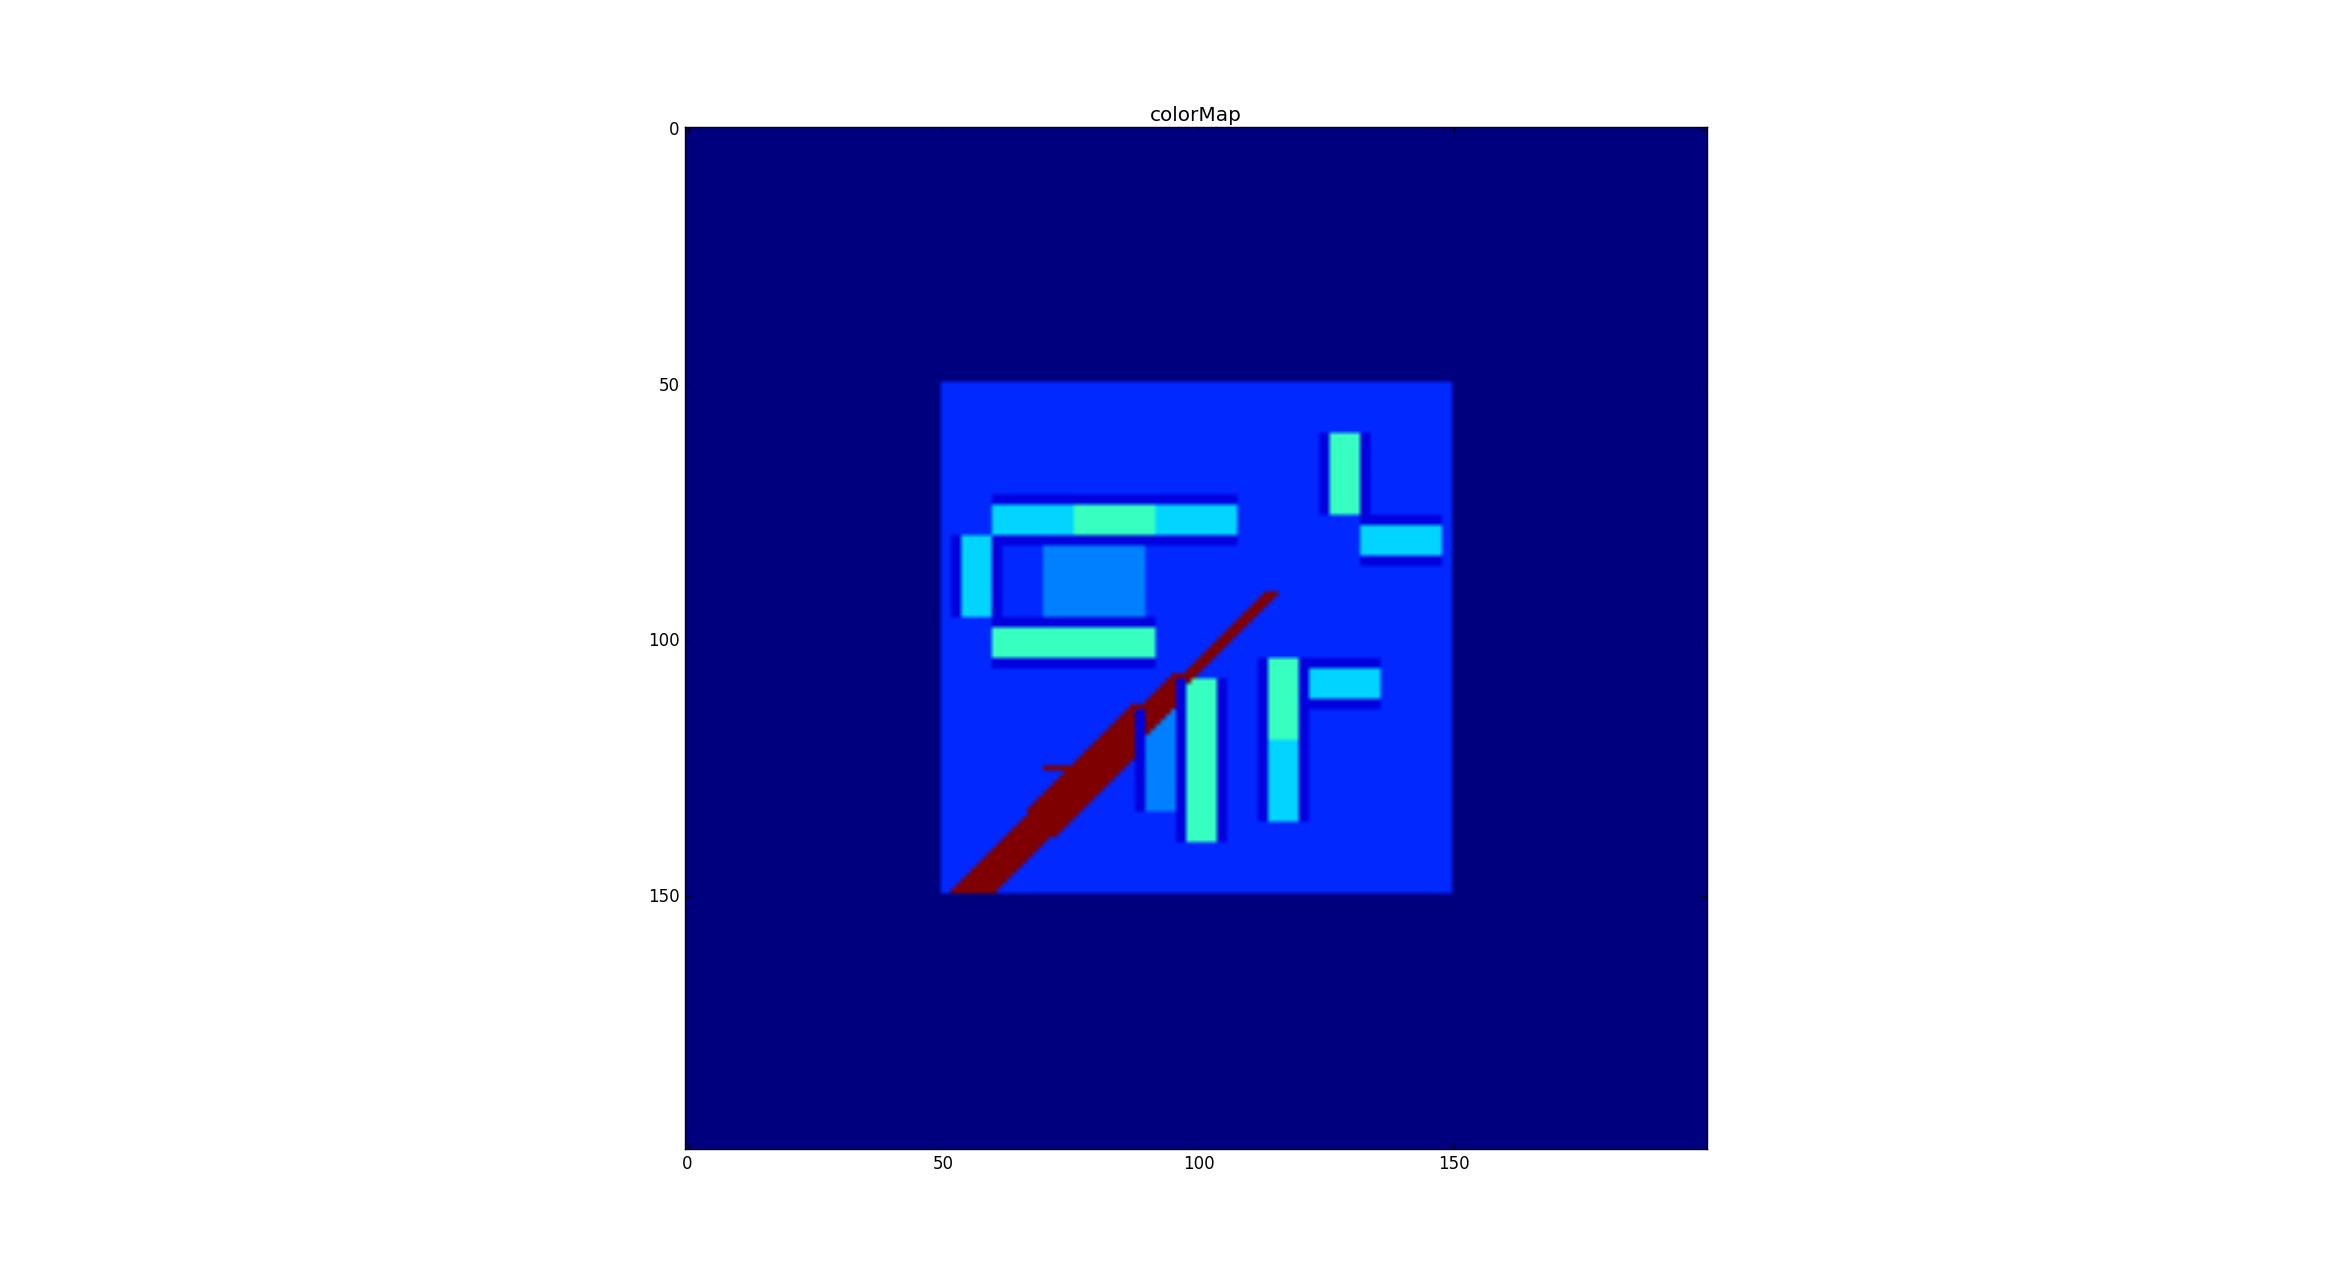
\includegraphics[width=0.5\textwidth]{pathAllocator}
  \caption{Greedy Best First Path Illuminated}
  \label{fig:gbf}
\end{figure}


\subsubsection{Role Switching}

As stated, the purpose of this research is to prove that subtask division can
be accomplished based on knowledge of robot capabilities. To test this at the
lowest level, each robot was given a set of terrains that they could maneuver through,
with no one being able to maneuver through walls. Terrain classification was set
in the following scheme and was recorded on the map nodes of the fullMap, which as
previously mentioned is hidden from view until the robots sense the cells in question.

\begin{tabularx}{\textwidth}{ |X|X|X|X|X| }
  \hline
  wall & open cell & ramp & small arch & large arch\\
  \hline
  -1  &  0  & 1  & 2 & 3 \\
  \hline
\end{tabularx}

Once a robot comes to an obstacle or region that it cannot maneuver around,
it will evaluate which team members are capable of doing so a request the
closest candidate to switch observable areas.
